\subsection{Архитектура CUDA}
\label{CUDA:section}
CUDA - архитектура параллельных вычислений на графических процессорах NVIDIA. Технология была представлена компанией в 2006 году. Подразумевалось, что новые компоненты снимут существующие тогда ограничения, а именно позволят использовать GPU для операций общего назначения, в том числе для вычислений с плавающей точкой. Но технология не сразу общедоступной, так как программистам все-еще приходилось маскировать вычисления под графические задачи. Для разрешения проблемы NVIDIA на базе языка С создала новый язык -- CUDA C, в котором появились ключевые слова, позволяющие управлять устройствами~\cite{KandrotSanders2022}.

\subsubsection*{Общие понятия, сборка и запуск приложения.} 
CUDA включает в себя расширение языка С (с элементами С++), набор оптимизированных библиотек, специальные драйверы CUDA. Позволяет увеличивать производительность вычислений благодаря использованию графических процессоров фирмы Nvidia.
Для разработки могут использоваться все основные операционные системы (Windows, Linux, MacOS).
При этом для написания программ возможно использование различных языков программирования. Первым был использован язык CUDA C - расширение языков С/C++, также можно использовать технологии OpenCL и DirectCompute. Кроме того, есть сторонние реализации для Java, Python, C\#.
Для разработки на CUDA необходимы следующие её составляющие:
\begin{itemize}
    \item\textbf{CUDA Driver} -- драйвер, обеспечивающий выполнение скомпилированных приложений на CUDA;
    \item\textbf{Cuda Toolkit} -- инструмент для разработки приложений, включающий в себя~\cite{Gergel2016}:
    \begin{itemize}
        \item Компилятор CUDA C NVCC (NVIDIA C Compiler);
        \item Оптимизированные библиотеки для графического процессора;
        \item Профилировщик;
        \item Драйвер CUDA Runtime;
        \item Документация.
    \end{itemize}
    \item\textbf{GPU Computing SDK} -- включает в себя некоторое количество примеров приложений для CUDA для базовых сценариев использования.
\end{itemize}

\subsubsection*{Преимущества CUDA}
\begin{itemize}
    \item Интерфейс основан на стандартном языке программирования C с некоторыми ограничениями, что упрощает изучение данной технологии;
    \item Более эффективные пересылки между памятью CPU и видеопамять;
    \item Полная поддержка целочисленных и побитовых операций;
    \item Разделяемая между потоками память (shared memory) размером в 16 Кб может быть использована под организованный пользователем кэш с более широкой полосой пропускания, чем при выборке из обычных текстур.
\end{itemize}

\subsubsection*{Ограничения CUDA}
\begin{itemize}
    \item Все функции, выполняемые на устройстве, не поддерживают рекурсии (в версии CUDA Toolkit 3.1 поддерживает указатели и рекурсию) и имеют некоторые другие ограничения;
    \item Неточные вычисления при работе с числами с плавающей запятой.
\end{itemize}

\subsubsection*{Программная модель CUDA} 
При создании программы CPU будет являться хостом (host), а GPU-ядром (kernel).

Рассмотрим внутреннюю программную модель CUDA, а также пример создания kernel-функции, исполняемой на устройстве.

\begin{figure}[H]
    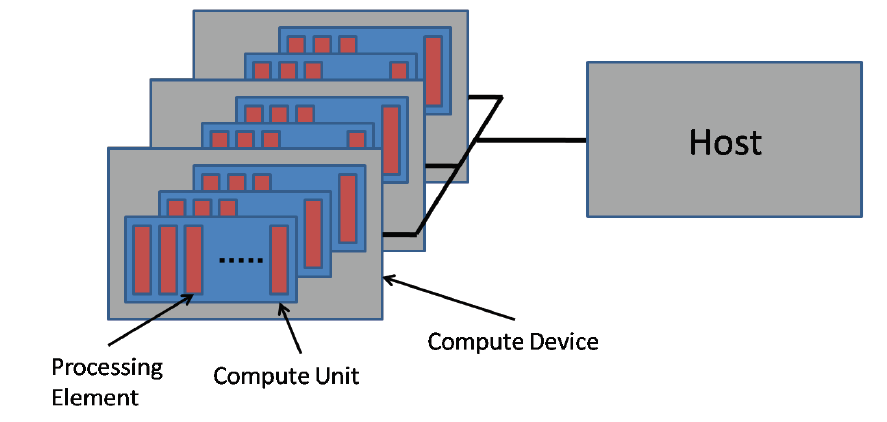
\includegraphics[width=\linewidth]{cuda/architecture}
    \caption{Архитектура CUDA}
    \label{CUDAArchitecture:image}
\end{figure}

Технология CUDA позволяет определять специальные функции – ядра (kernels), которые выполняются параллельно на ГПУ в виде множества различных потоков (threads). Таким образом, ядро является аналогом потоковой функции. Каждый поток исполняется на одном CUDA-ядре, используя собственный стек инструкций и локальную память. Отдельные потоки группируются в блоки потоков (thread block) одинакового размера, при этом каждый блок потоков выполняется на отдельном мультипроцессоре.
На аппаратном уровне потоки блока группируются в так называемые варпы (warps) по 32 элемента (на всех текущих устройствах), внутри которых все потоки параллельно выполняют одинаковые инструкции (по принципу SIMD\footnote{SIMD -- Single Instruction, Multiple Data}).
В свою очередь, блоки потоков объединяются в решетки блоков потоков (grid of thread blocks). Взаимодействие потоков из разных блоков во время работы ядра затруднено: отсутствуют явные инструкции синхронизации, взаимодействие возможно через глобальную память и использованием атомарных функций (другим вариантом является разбиение ядра на несколько ядер без внутреннего взаимодействия между потоками разных блоков).
Каждый поток внутри блока потоков имеет свои координаты (одно-, двух- или трехмерные), которые доступны через встроенную переменную \texttt{threadIdx}. В свою очередь, координаты блока потоков (одно-, двух- или трехмерные) внутри решетки определяются встроенной переменной \v{blockIdx}. Данные встроенные переменные являются структурами с полями \texttt{.x}, \texttt{.y}, \texttt{.z}.

Встроенные переменные-векторы:
\begin{itemize}
    \item\code[text]{uint3 threadIdx} -- индекс нити в блоке
    \item\code[text]{dim3 blockDim} -- размеры блока
    \item\code[text]{uint3 blockIdx} -- индекс блока в сетке
    \item\code[text]{dim3 gridDim} -- размеры сетки
\end{itemize}

\noindentЛинейный индекс потока (одномерный случай): 
\mint{cuda}{int tid = blockIdx.x * blockDim.x + threadIdx.x;}

\noindentОбщее количество потоков (одном. случай): 
\mint{cuda}{int threads_total = blockDim.x * gridDim.x;}

\textbf{Kernel-функция.} Пример создания функции и вызов ее с device:
\begin{minted}{cuda}
__global__ void kernel_function(float* data) { ... }

kernel_function<<<blocks, threads, nshared, stream>>> (data);
\end{minted}

Используемые параметры:
\begin{itemize}
    \item\texttt{blocks (grid)} -- задает число блоков
    \item\texttt{threads (block)} -- задает число нитей в блоке
    \item\texttt{nshared} -- количество дополнительной shared- памяти, выделяемое блоку \textit{(необязательный параметр)}
    \item\texttt{stream} -- номер потока CUDA, в котором нужно запустить ядро \textit{(необязательный параметр)}
\end{itemize}

Создаётся \texttt{blocks * threads} вычислительных нитей в процессе выполнения функции.

\textbf{Определение размера параметров.} Оба параметра представляют собой вектор из трёх координат. В CUDA есть функция,с помощью которой можно вычислить размер блоков, а также формула для размера грида.

\noindentФункция для определения подходящего blockSize:
\mint{cuda}{cudaOccupancyMaxPotentialBlockSize(&minGridSize, func_name, 0, N);}

\noindentФормула для gridSize:
\mint{cuda}{gridSize = (N + blockSize - 1) / blockSize;}

\textbf{Используемые идентификаторы.} Для определения памяти используется три идентификатора - device, global и host.

Device выполняется на устройстве, вызываться может также только там. global, с которым обычно и создаются функции, можно вызвать откуда угодно, а выполняться будет всё на устройстве. И по умолчанию всегда ставится host, который выполняется на CPU и вызывается оттуда же.

\begin{table}[H]
    \begin{tabularx}{\textwidth}{|c|C|C|}
    \hline
                    & \textbf{Можно вызвать с}   & \textbf{Выполняется на}     \\ \hline
    \texttt{\_\_device\_\_}  & device            & device         \\ \hline
    \texttt{\_\_global\_\_}  & host, device      & device         \\ \hline
    \texttt{\_\_host\_\_}    & host              & host           \\ \hline
    \end{tabularx}
\end{table}

Для переменных также есть device. Кроме него есть ещё constant для констант и shared для общей памяти между блоками.

\begin{table}[H]
    \begin{tabularx}{\textwidth}{|c|C|C|}
    \hline
                    & \textbf{Расположение в памяти} & \textbf{Область видимости} \\ \hline
    \texttt{\_\_device\_\_}      & device (global)       & сетка \\ \hline
    \texttt{\_\_constant\_\_}    & device (constant)     & сетка \\ \hline
    \texttt{\_\_shared\_\_}      & device (shared)       & блок  \\ \hline
    \end{tabularx}
\end{table}

\subsubsection*{Структура памяти CUDA}
Виды памяти в CUDA:
\begin{itemize}
    \item Локальная (local)
    \item Разделяемая (shared)
    \item Глобальная (global)
    \item Память констант (constant)
    \item Текстурная (texture)
\end{itemize}

Каждый поток обладает своей локальной памятью (local memory).
Все потоки внутри блока имеют доступ к быстрой разделяемой памяти блока (shared memory), время жизни которой совпадает со временем жизни блока. Разделяемая память блока разбита на страницы, при этом доступ к данным на разных страницах осуществляется параллельно.

Все потоки во всех блоках имеют доступ к глобальной памяти устройства (global memory или device memory), которая всегда хранит своё состояние во время работы программы.

Всем потокам также доступны два вида общей кэшируемой памяти для чтения: константная (constant) и текстурная (texture). Так же как и в глобальной памяти устройства, данные хранятся всегда во время работы программы. При этом текстурная память обеспечивает различные режимы адресации и поддерживает фильтрацию для определенных форматов данных. Фильтрация реализована на аппаратном уровне и может эффективно использоваться в различных задачах \cite{Gergel2016}.

\begin{figure}[H]
    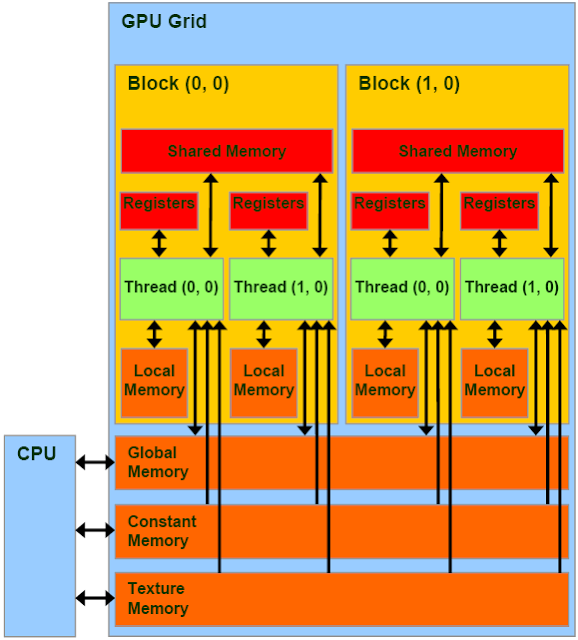
\includegraphics[width=\linewidth]{cuda/memory}
    \caption{CUDA. Структура памяти}
    \label{CudaMemory:image}
\end{figure}

\subsubsection*{Основные функции CUDA для работы с памятью}
В CUDA основными функциями являются функции для выделения и очистки памяти, а также пересылка данных между устройствами.
\begin{itemize}
    \item\texttt{cudaError\_t cudaMalloc(void **devPtr, size\_t size)} -- поз\-во\-ля\-ет выделить память на GPU размером \texttt{size} с указателем на \texttt{devPtr}. Возвращает код из структуры \texttt{cudaError\_t}, в котором будет код успеха или один из многочисленных кодов ошибок с описанием.
    \item\texttt{cudaError\_t cudaFree(void *devPtr)} - позволяет очистить область памяти, на которую указывает \texttt{devPtr}. Возвращает код из структуры \texttt{cudaError\_t}, в котором будет код успеха или один из многочисленных кодов ошибок с описанием.
    \item\texttt{cudaError\_t cudaMemcpy(void *dst, const void *src, \\ size\_t size, enum cudaMemcpyKind kind)} - позволяет скопировать данные размера size с источника \texttt{src} на получателя \texttt{dst}. Возвращает код из структуры \texttt{cudaError\_t}, в котором будет код успеха или один из многочисленных кодов ошибок с описанием. Последний параметр \texttt{kind} показывает, куда и откуда необходимо отправить данные, принимает следующие значения:
    \begin{itemize}
        \item \texttt{cudaMemcpyHostToHost} -- копирование с CPU на CPU
        \item \texttt{cudaMemcpyHostToDevice} -- копирование с CPU на GPU
        \item \texttt{cudaMemcpyDeviceToHost} -- копирование с GPU на CPU
        \item \texttt{cudaMemcpyDeviceToDevice} -- копирование с GPU на GPU
        \item \texttt{cudaMemcpyDefault} -- позволяет не указывать направление, поскольку оно может быть вычислено по принадлежности указателей.
    \end{itemize}
\end{itemize}

\subsubsection*{Синхронизация событий}
Для каждой многопоточной программы необходимо синхронизация потоков перед выполнением каких-либо нераспараллеленных действий или при доступе к общему ресурсу. В CUDA есть возможность синхронизации потоков с использованием cuda-event, которое работает аналогично барьерам.

Необходимо создать и записать события, а потом вызывать функцию синхронизации в нужном месте программы, где все потоки будут ожидать завершения остальных. Также в конце программы необходимо удалить данное событие.

Используемые функции:
\begin{itemize}
    \item \texttt{cudaEvent\_t syncEvent} -- создание переменной для events;
    \item \texttt{cudaEventCreate(\&syncEvent)} -- создание и инициализация \linebreak event;
    \item \texttt{cudaEventRecord(syncEvent, nullptr)} -- запись этого события барьера, чтобы все потоки о нём узнали;
    \item \texttt{cudaEventSynchronize(syncEvent)} -- метка синхронизации, то есть место, где потоки должны ожидать выполнения друг друга;
    \item \texttt{cudaEventDestroy(syncEvent)} -- удаление event.
\end{itemize}

Описанный выше пример подходит для синхронизации на host. Но также есть функции, которые можно вызывать на самом устройстве~\cite{CudaSyncHabr}:
\begin{itemize}
    \item\texttt{\_\_syncthreads()} -- функция заставит каждый поток ждать, пока все остальные потоки этого блока достигнут этой точки и все операции по доступу к разделяемой и глобальной памяти, совершенные потоками этого блока, завершатся и станут видны потокам этого блока.
    \item\texttt{\_\_threadfence\_block()} -- будет заставлять ждать вызвавший её поток, пока все совершенные операции доступа к разделяемой и глобальной памяти завершатся и станут видны потокам этого блока.
    \item\texttt{\_\_threadfence()} -- будет заставлять ждать вызвавший её поток, пока все совершенные операции доступа к разделяемой памяти станут видны потокам этого блока, а операции с глобальной памятью — всем потокам на графическом устройстве.
    \item\texttt{\_\_threadfence\_system()} -- подобна \texttt{\_\_threadfence()}, но включает синхронизацию с потоками на CPU, при использовании весьма удобной page-locked памяти.
\end{itemize}

\subsubsection*{Управление устройствами}
В CUDA представлен простой интерфейс, позволяющий узнать какие устройства с какими параметрами есть в системе. Примерами таких функций служат:
\begin{itemize}
    \sloppy
    \item\texttt{cudaError\_t cudaGetDeviceCount(int *count)} -- получение числа доступных устройств;
    \item\texttt{cudaError\_t cudaGetDevice(int *dev)} -- получение номера текущего используемого устройства;
    \item\texttt{cudaError\_t cudaGetDeviceProperties(struct cudaDeviceProp *prop, int dev)} -- заполнение структуры, содержащей свойства устройства;
    \item\texttt{cudaError\_t cudaChooseDevice(int *dev, const struct cudaDeviceProp *prop)} -- выбор устройства, которое лучше всего соответствует переданной конфигурации;
    \item\texttt{cudaError\_t cudaSetDevice(int dev)} -- установка определённого устройства.
\end{itemize}

Сначала полезно узнать сколько всего устройств при помощи функции \texttt{cudaGetDeviceCount}:
\begin{minted}{cuda}
int count;
cudaDeviceProp prop; 
cudaGetDeviceCount(&count);
\end{minted}

Далее итеративно можно прочитать параметры каждого устройства:
\begin{minted}{cuda}
for (int i=0; i<count; ++i)
    cudaGetDeviceProperties(&prop, i);
\end{minted}

С полным списком параметров в структуре \texttt{cudaDeviceProp} можно ознакомится в документации: \url{https://docs.nvidia.com/cuda/cuda-runtime-api/structcudaDeviceProp.html}.

\subsubsection*{Обработка ошибок}
Каждая CUDA-функция возвращают структуру \code[cuda]{cudaError_t}, за счёт которой можно понять, успешно ли произошло, например, выделение памяти. Примеры кодов возврата:
\begin{itemize}
    \item\code[cuda]{cudaSuccess} -- при успешном завершении
    \item\code[cuda]{cudaErrorInvalidValue} -- неправильно переданный аргумент при вызове CUDA-функции
    \item\code[cuda]{cudaErrorMemoryAllocation} -- ошибка выделения памяти
    \item\code[cuda]{cudaErrorInitializationError} -- невозможно вызвать функцию, поскольку CUDA driver не проинициализирован
\end{itemize}

Кроме того, есть функция для получения последней брошенной ошибки для её последующей обработки в нужном месте программы (также возвращает код ошибки из \code[cuda]{cudaError_t}).

\mint{cuda}{cudaError_t error = cudaGetLastError();}

\subsubsection*{Пример программы}
\begin{minted}{cuda}
__global__ void proccess_smth(double* arr, int size) { 
    // calculating something
}

int main(int argc, char *argv[]) {
    // prepare array arr by host
    // allocate bytes on device
    size_t arr_size = sizeof(double) * N;
    cudaMalloc(&arr_gpu, v);
    
    // copy to device
    cudaMemcpy(arr_gpu, arr, arr_size, cudaMemcpyHostToDevice);
    proccess_smth<<<gridSize, blockSize>>>(arr_gpu, N);()
    
    // copy result to host
    cudaMemcpy(arr, arr_gpu, arr_size, cudaMemcpyDeviceToHost); 
    cudaFree(arr_gpu) ;
    ...
}
\end{minted}

При использовании синхронизации код преобразуется следующим образом:
\begin{minted}{cuda}
int main(int argc, char *argv[]) {
    // define event to synchronize host & device 
    cudaEvent_t syncEvent;
    cudaEventCreate(&syncEvent); 
    cudaEventRecord(syncEvent, nullptr);
    
    proccess_smth<<<gridSize, blockSize>>>(arr_gpu, N);()
    
    cudaEventSynchronize(syncEvent);
    ... 
}
\end{minted}

\subsubsection*{Профилирование}
Вместе с CUDA обычно поставляется также отдельный профилировщик. NVVP\footnote{NVIDIA Visual Profiler} -- визуальная составляющая базового профилировщика. Пример интерфейса основного окна представлен на рисунке~\ref{CudaProfiling:image}.

\begin{figure}[H]
    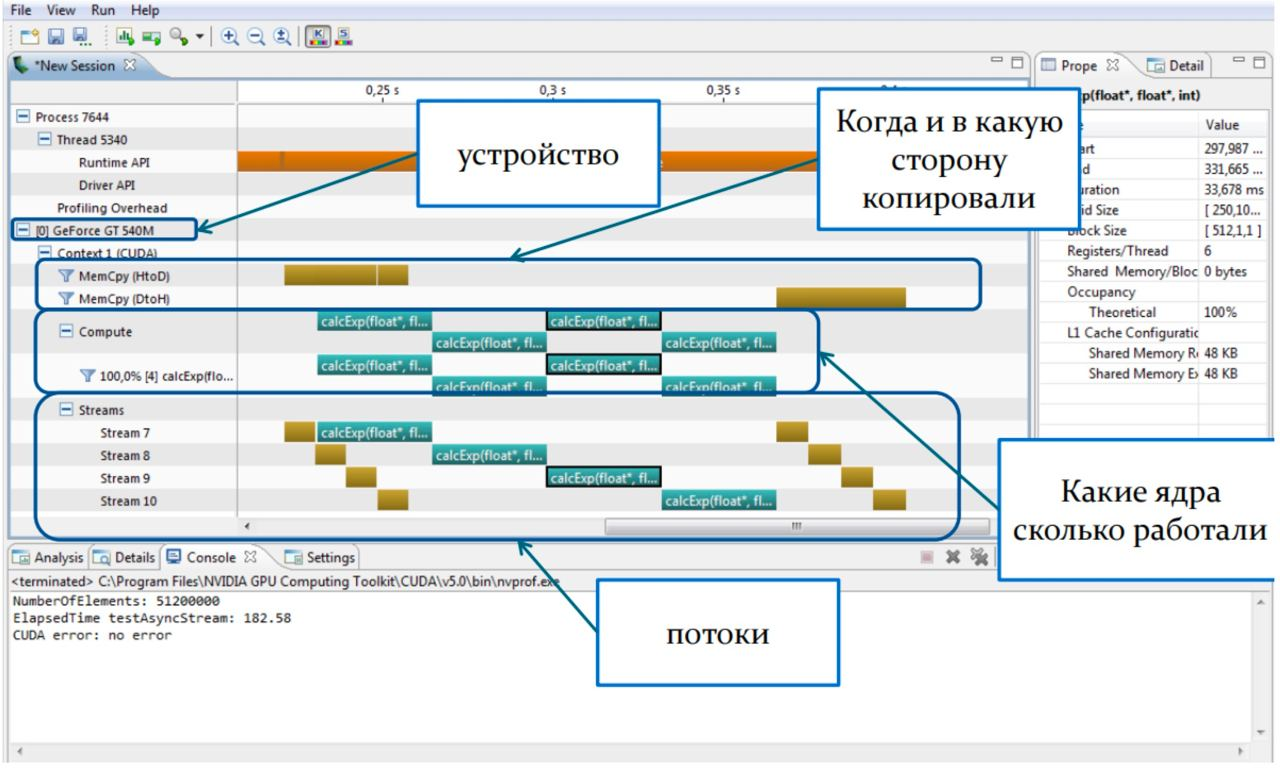
\includegraphics[width=\linewidth]{cuda/profiling_app}
    \caption{Пример интерфейса профилировщика CUDA}
    \label{CudaProfiling:image}
\end{figure}

\noindentКоманда для профилирования:
\mint{text}{nvprof [options] [application] [application-arguments]}

\noindentПример команды:
\mint{text}{nvprof --unified-memory-profiling per-process-device ./program}

\noindentПример вывода: \\
\noindent\resizebox{\textwidth}{!}{
    \begin{tabular}{|rrrrrrl|}
        \hline
        \multicolumn{7}{|l|}{==5286== NVPROF is profiling process 5286, command: ./program [args]} \\
        \multicolumn{7}{|l|}{==5286== Profiling application: ./program [args]} \\
        \multicolumn{7}{|l|}{==5286== Profiling result:} \\
        \textbf{Time(\%)} & \textbf{Time} & \textbf{Calls} & \textbf{Avg} & \textbf{Min} & \textbf{Max} & \textbf{Name} \\
        26.47\% & 639.68us & 100 & 6.41us & 6.01us & 16.2us & func1(double*, double*, int) \\
        22.99\% & 555.58us & 100 & 5.55us & 5.50us & 7.13us & func2(double*, int) \\
        18.48\% & 446.68us & 300 & 1.49us & 1.21us & 9.08us & [CUDA memcpy HtoD] \\
        16.27\% & 393.29us & 100 & 3.93us & 3.65us & 12.1us & func3(double const *, double*, int) \\
        15.78\% & 381.40us & 300 & 1.27us & 1.09us & 2.43us & [CUDA memcpy DtoH] \\
        \hline
    \end{tabular}
}

\texttt{{\textendash\textendash}unified-memory-profiling per-process-device} -- общее потребление памяти и время выполнения вызываемых функций. per-process-device расписывает для каждого процесса.

Также в выводе можно увидеть общее, минимальное, максимальное и среднее (суммарное) время работы для каждой функции устройства, а также затраты на копирование данных с CPU на GPU и обратно.

\texttt{{\textendash\textendash}print-gpu-trace} -- печатать более детальную информацию по каждому запуску kernel и отсортировать в хронологическом порядке.

\subsubsection*{Сравнение CUDA и OpenCL}
Достоинство OpenСL -- открытый стандарт, программы будут работать на любом устройстве поддерживающем этот стандарт, в том числе на CPU. С другой стороны исходные программы, использующие OpenCL состоят из двух экземпляров: основная программа (для CPU) и текст для OpenCL. Соответственно, при внесении изменений всегда требуется поддерживать актуальными оба экземпляра. CUDA с этой точки зрения - полная противоположность OpenCL, так как, с одной стороны выполняется только на GPU от NVIDIA, с другой стороны, ограничивается наличием единого исходного текста - файла с расширением .cu.

Программа, использующая OpenCL может быть запущена на ряде слабосвязанных устройств, хотя потребуются дополнительные усилия, чтобы реализовать программу таким образом, чтобы минимизировать привязку к конкретному устройству. Ядро OpenCL может быть скомпилировано во время выполнения, хотя это отрицательно скажется на скорости. CUDA, в силу того, что разрабатывается той же компанией, что и аппаратное обеспечение может представить лучшую производительность, но в общем случае это зависит от качества кода, выполняемой задачи и используемых алгоритмов.

CUDA -- проприетарный фреймворк NVIDIA, в то время как у OpenCL окрыт исходный код. Хотя комьюнити CUDA больше, она чаще обсуждается на форумах, обладает большей документацией и считается более простой для понимания и изучения. Тем не менее комьюнити OpenCL растет с каждым годом.

OpenCL будет работать на любой ОС, в то время как CUDA будет работать только на ведущих ОС, с условием использования NVIDIA.

Для CUDA существуют много высокопроизводительных библиотек, для OpenCL их меньше~\cite{Krasnov2002}.

\subsubsection*{Сферы применения CUDA}
\textbf{Обработка медицинских изображений.} В данной сфере есть несколько проблем. При проведении исследований (УЗИ, МРТ и др.) необходимо быстро получать, обрабатывать и сохранять большие объемы данных. Сложность в том, что использовать сжатие - крайне нежелательно. Раньше подобные исследования были слишком дорогими для клинического исследования, а следовательно, страдали люди, которые пропустили первые стадии серьезных заболеваний. CUDA позволила разрешить проблему быстрой обработки больших объемов информации, что сделало исследования более доступными. Это в свою очередь положительно сказалось на постановке диагнозов и лечении пациентов с онкологическими заболеваниями.

\textbf{Вычислительная гидродинамика.} Для проектирования эффективных винтов и лопаток необходимо проведение экспериментов со сложными численными моделями, так как требуется анализ сложного движения воздуха и жидкости, обтекающих винты и лопатки. CUDA сделала подобные исследования более доступными, сегодня частичные результаты доступны уже через несколько секунд.

\textbf{Окружающая среда.} Проблема возникла около чистящих сре\-дств, а именно их компонентами - ПАВ (поверхностно-активными веществами), которые отвечают за эффективность средства. ПАВ хорошо сцепляется с частицами грязи, а также с частицами воды. Проблема в том, что эффективность часто сопровождается пагубным воздействием на окружающую среду. Поэтому требуется проведение экспериментов по варьированию комбинаций компонентов и загрязнений, чтобы опередить наиболее эффективный и наименее вредный состав. Данная задача может быть разрешена с использованием CUDA.